% begin module MVT-meaning
\begin{frame}[t]
\begin{theorem}[The Mean Value Theorem]
Let $f$ be a function that is continuous on $[a,b]$ and differentiable on $(a,b)$. 
Then there is a number $c$ in $(a,b)$ such that $f'(c) = \frac{f(b)-f(a)}{b-a}$.
\end{theorem}
\begin{columns}[c]
\column{.5\textwidth}
\ \only<handout:0| -4>{%
\uncover<2->{%
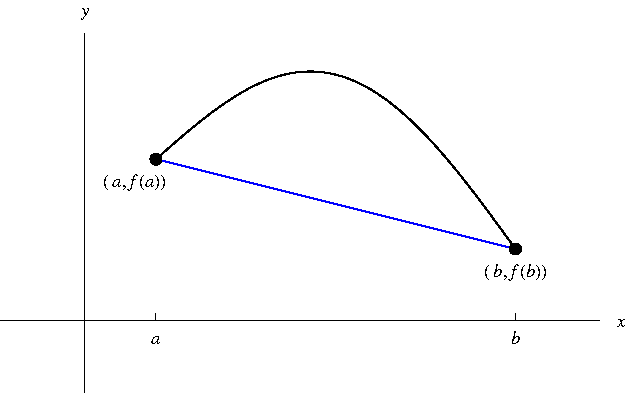
\includegraphics[height=4cm]{maxima-minima/pictures/04-02-mvta.pdf}%
}%
}%
\only<handout:1| 5>{%
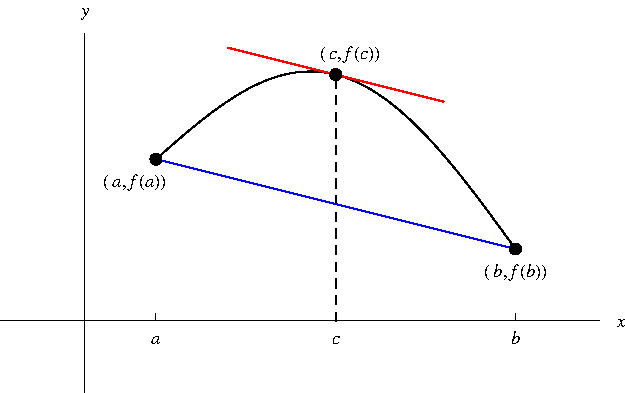
\includegraphics[height=4cm]{maxima-minima/pictures/04-02-mvtb.pdf}%
}%
\only<handout:2| 6->{%
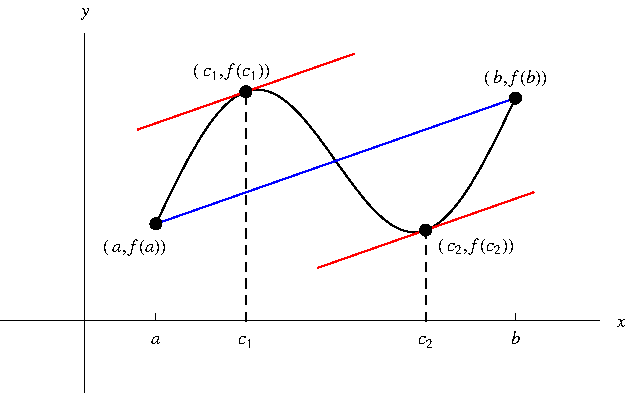
\includegraphics[height=4cm]{maxima-minima/pictures/04-02-mvtc.pdf}%
}%
\column{.5\textwidth}
\begin{itemize}
\item<2->  Consider the secant line from $(a, f(a))$ to $(b, f(b))$.
\item<2-| alert@3-4>  Slope: $m = $ \uncover<4->{$\frac{f(b)-f(a)}{b-a}$.}
\item<5->  The Mean Value Theorem says somewhere in $(a,b)$ is a number $c$ where the slope of the tangent equals $m$.
\item<handout:2| 6->  Maybe more than one number.
\end{itemize}
\end{columns}
\end{frame}
% end module MVT-meaning
